\section{Definitions}
\subsection{Ranking, bipartite ranking and pairwise bipartite ranking}

\begin{frame}{Ranking}

    {\large\textbf{What is ranking ?}}
    
    Ranking is a class of machine learning algorithms aiming to \gbf{sort} a list of observations according to some \gbf{criterion}. 
    
    \vspace{0.3cm}
    
    {\large\textbf{Examples}}
    
    \begin{itemize}
        \item Information retrieval : Sort documents according to their relevance to a query
        \item Recommendation systems : Recommend user's favourite songs first
    \end{itemize}
\end{frame}

% \begin{frame}{Ranking}
%     \begin{figure}[H]
%         \centering
%         \begin{tikzpicture}
%             \begin{axis}[ 
%                 xlabel=x,
%                 ylabel=y,
%                 xmin=0, xmax=1.0,
%                 ymin=0, ymax=1.0,
%                 xtick={0,0.2,0.4,0.6,0.8,1.0},
%                 ytick={0,0.2,0.4,0.6,0.8,1.0},
%                 legend pos=outer north east,
%                 height=0.4\textwidth,
%                 label style={font=\small},
%                 tick label style={font=\small},
%                 legend cell align={left},
%                 legend style={font=\footnotesize,
%                             cells={align=left}}
%                 ] 
%                 \centering
%                 \addplot
%                 coordinates {(0.12,0.36)(0.15,0.33)(0.11,0.48)(0.6,0.45)};
%                 \addlegendentry{ROC curve for perfect model};
%             \end{axis}
%         \end{tikzpicture}
%     \end{figure}
% \end{frame}

\begin{frame}{Bipartite ranking}

    {\large\textbf{What is bipartite ranking ?}}
    
    In bipartite ranking, we consider that all the observations that we want to sort can be partitioned into two classes : \gbf{positive} and \gbf{negative}. We want the positive instances to be consistently \gbf{ranked higher} than the negative ones.
    
    \vspace{0.3cm}

    {\large\textbf{Examples}}
    
    \begin{itemize}
        \item Fraud detection : Find the observations that are most likely to be fraudulent among fraudulent and non-fraudulent observations
        \item Recommendation systems : Recommend user's favourite songs first but this time we have songs that are liked by the user and songs that are disliked
    \end{itemize}
\end{frame}

\begin{frame}{Bipartite ranking}

    {\large\textbf{What is the difference between bipartite ranking and binary classification ?}}

    Bipartite ranking is very close to binary classification since we are trying to distinguish positive instances from negative instances, but \gbf{serves a slightly different goal}. In the cases where a model needs to process a \gbf{large number of observations} and where a \gbf{human verification is needed}, a bipartite ranking model would be able to provide the \gbf{most likely positive instances} first, allowing the human to only investigate a limited number of instances.
    
\end{frame}

\begin{frame}{Bipartite ranking}

    {\large\textbf{What is the difference between bipartite ranking and binary classification ?}}

    There are some works \footcite{narasimhan2013relationship} working around the \gbf{link} between the two that were able to show that a \gbf{good ranking model}, once \gbf{transferred to binary classification}, will perform \gbf{well} (provided that the right threshold was found), while the \gbf{opposite is not always true}. 

    \begin{figure}
        \centering
        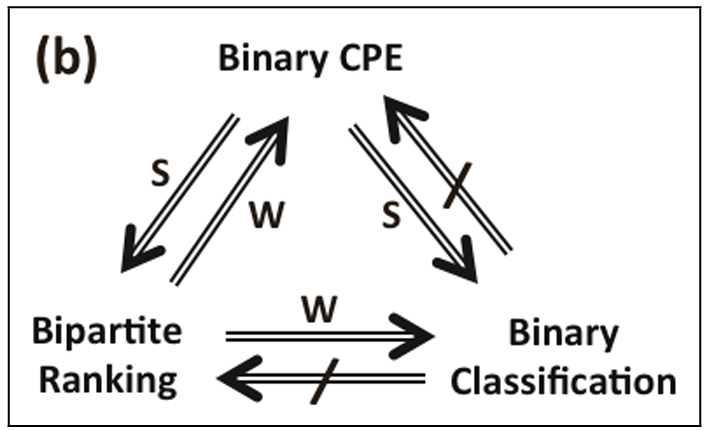
\includegraphics[scale=0.3]{images/link.png}
    \end{figure}
    
\end{frame}

\begin{frame}{Pairwise bipartite ranking}

    {\large\textbf{What is pairwise bipartite ranking ?}}

    Pairwise bipartite ranking is specific case of bipartite ranking, in which we rank each instance \gbf{relatively to another instance}.  Instead of simply distinguishing between positive and negative items, pairwise bipartite ranking considers the \gbf{relative preference between pairs of items}. 

    \vspace{0.3cm}

    {\large\textbf{Example}}
    
    \begin{itemize}
        \item Facial recognition : Find pairs of faces that are the most similar in a database
    \end{itemize}

    \textit{(This is not the focus of this presentation, but this is what I'm currently working on.)}

    
\end{frame}


\subsection{ROC curve and AUC}
\begin{frame}{ROC curve}
    
    {\large\textbf{What is a ROC curve ?}}
    
    ROC stands for \gbf{Receiver Operating Characteristic} curve and is a graph showing the performance of a classification model \gbf{at all classification thresholds}. It plots the false positive rate in the x-axis against the true positive rate in the y-axis. 

    \begin{figure}
        \centering
        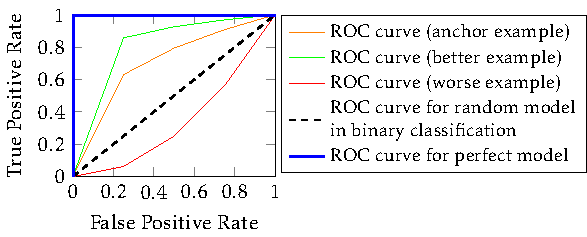
\includegraphics[page=1, scale=0.9]{images/output-figure0.pdf}
        \vspace{-0.3cm}
        \caption{Different ROC curves}
    \end{figure}

    \vspace{-0.4cm}

    \tiny{Warning : When a curve is below the diagonal (like for the red line), we can simply switch the labels of the classes and we will get a better model. This means that the worst possible model is actually the random model.}\par
    
    % \begin{figure}[H]
    %     \centering
    %     \begin{tikzpicture}
    %         \begin{axis}[ 
    %             xlabel=False Positive Rate,
    %             ylabel=True Positive Rate,
    %             xmin=0, xmax=1.0,
    %             ymin=0, ymax=1.0,
    %             xtick={0,0.2,0.4,0.6,0.8,1.0},
    %             ytick={0,0.2,0.4,0.6,0.8,1.0},
    %             legend pos=outer north east,
    %             height=0.4\textwidth,
    %             label style={font=\small},
    %             tick label style={font=\small},
    %             legend cell align={left},
    %             legend style={font=\footnotesize,
    %                         cells={align=left}}
    %           ] 
    %             \centering 
    %             \addplot[domain=0:1,
    %             samples=5, color = orange]{x^(1/3)};
    %             \addlegendentry{ROC curve (anchor example)};
    %             \addplot[domain=0:1,
    %             samples=5, color = green]{x^(1/9)};
    %             \addlegendentry{ROC curve (better example)};
    %             \addplot[domain=0:1,
    %             samples=5, color = red]{x^2};
    %             \addlegendentry{ROC curve (worse example)};
    %             \addplot[domain=0:1,
    %             samples=10, color = black, thick, dashed]{x};
    %             \addlegendentry{ROC curve for random model \\in binary classification};
    %             \addplot[domain=0:1,
    %             color = blue, {very thick}]
    %             coordinates {(0,0)(0,1)(1,1)};
    %             \addlegendentry{ROC curve for perfect model};
    %       \end{axis}
    %     \end{tikzpicture}
    %     \caption{Different ROC curves}
    % \end{figure}
    
        
\end{frame}


\begin{frame}{AUC}
    
    {\large\textbf{What is the AUC ?}}
    
    AUC stands for \gbf{Area Under the Curve} and is a widely used metric for machine learning model evaluation that quantifies the overall performance of the model \gbf{across all possible classification thresholds}. AUC measures the entire two-dimensional area underneath the entire ROC curve from (0,0) to (1,1). 
    
    {\large\textbf{Example}}
    \begin{itemize}
    	\item A model who is 100\% wrong has an AUC of 0.
    	\item A model who is 100\% correct has an AUC of 1.
    
    \end{itemize}
    
\end{frame}

\begin{frame}{AUC}
    
    {\large\textbf{What is the AUC ?}}

    \begin{figure}
        \centering
        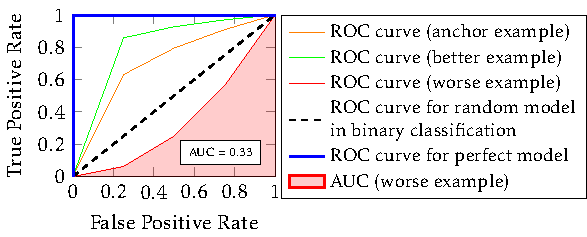
\includegraphics[page=1]{images/output-figure1.pdf}
        \caption{AUC for the worst ROC curve}
    \end{figure}

    
    % \begin{figure}[H]
    %     \centering
    %     \begin{tikzpicture}
    %         \begin{axis}[ 
    %             xlabel=False Positive Rate,
    %             ylabel=True Positive Rate,
    %             xmin=0, xmax=1.0,
    %             ymin=0, ymax=1.0,
    %             xtick={0,0.2,0.4,0.6,0.8,1.0},
    %             ytick={0,0.2,0.4,0.6,0.8,1.0},
    %             legend pos=outer north east,
    %             height=0.4\textwidth,
    %             label style={font=\small},
    %             tick label style={font=\small},
    %             legend cell align={left},
    %             legend style={font=\footnotesize,
    %                         cells={align=left}}
    %           ] 
    %             \centering 
    %             \path[name path=axis] (axis cs:0,0) -- (axis cs:1,0);
    %             \addplot[domain=0:1,
    %             samples=5, color = orange]{x^(1/3)};
    %             \addlegendentry{ROC curve (anchor example)};
    %             \addplot[domain=0:1,
    %             samples=5, color = green]{x^(1/9)};
    %             \addlegendentry{ROC curve (better example)};
    %             \addplot[domain=0:1,
    %             samples=5, color = red, name path=worse_roc]{x^2};
    %             \addlegendentry{ROC curve (worse example)};
    %             \addplot[domain=0:1,
    %             samples=10, color = black, thick, dashed]{x};
    %             \addlegendentry{ROC curve for random model \\in binary classification};
    %             \addplot[domain=0:1,
    %             color = blue, {very thick}]
    %             coordinates {(0,0)(0,1)(1,1)};
    %             \addlegendentry{ROC curve for perfect model};
    %             \addplot [
    %                 thick,
    %                 color=red,
    %                 fill=red, 
    %                 fill opacity=0.2
    %             ]
    %             fill between[
    %                 of=worse_roc and axis,
    %                 soft clip={domain=0:1},
    %             ];
    %             \addlegendentry{AUC (worse example)};
    %             \node[font=\tiny,fill=white,draw,rectangle] at (axis cs: 0.73,0.15) {AUC = 0.33};
    %       \end{axis}
    %     \end{tikzpicture}
    %     \caption{AUC for the worst ROC curve}
    % \end{figure}


\end{frame}

\begin{frame}{AUC}
    
    {\large\textbf{What is the AUC ?}}

    \begin{figure}
        \centering
        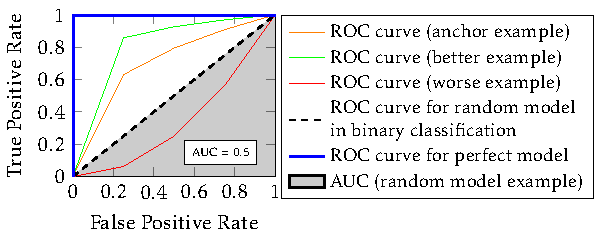
\includegraphics[page=1]{images/output-figure2.pdf}
        \caption{AUC for the random model ROC curve}
    \end{figure}

    % \begin{figure}[H]
    %     \centering
    %     \begin{tikzpicture}
    %         \begin{axis}[ 
    %             xlabel=False Positive Rate,
    %             ylabel=True Positive Rate,
    %             xmin=0, xmax=1.0,
    %             ymin=0, ymax=1.0,
    %             xtick={0,0.2,0.4,0.6,0.8,1.0},
    %             ytick={0,0.2,0.4,0.6,0.8,1.0},
    %             legend pos=outer north east,
    %             height=0.4\textwidth,
    %             label style={font=\small},
    %             tick label style={font=\small},
    %             legend cell align={left},
    %             legend style={font=\footnotesize,
    %                         cells={align=left}}
    %           ] 
    %             \centering 
    %             \path[name path=axis] (axis cs:0,0) -- (axis cs:1,0);
    %             \addplot[domain=0:1,
    %             samples=5, color = orange]{x^(1/3)};
    %             \addlegendentry{ROC curve (anchor example)};
    %             \addplot[domain=0:1,
    %             samples=5, color = green]{x^(1/9)};
    %             \addlegendentry{ROC curve (better example)};
    %             \addplot[domain=0:1,
    %             samples=5, color = red, name path=worst_roc]{x^2};
    %             \addlegendentry{ROC curve (worse example)};
                
    %             \addplot[domain=0:1,
    %             samples=10, color = black, thick, dashed, name path=random_roc]{x};
    %             \addlegendentry{ROC curve for random model \\in binary classification};
    %             \addplot[domain=0:1,
    %             color = blue, {very thick}]
    %             coordinates {(0,0)(0,1)(1,1)};
    %             \addlegendentry{ROC curve for perfect model};
    %             \addplot [
    %                 thick,
    %                 color=black,
    %                 fill=black, 
    %                 fill opacity=0.2
    %             ]
    %             fill between[
    %                 of=random_roc and axis,
    %                 soft clip={domain=0:1},
    %             ];
    %             \addlegendentry{AUC (random model example)};
    %             \node[font=\tiny,fill=white,draw,rectangle] at (axis cs: 0.73,0.15) {AUC = 0.5};
    %       \end{axis}
    %     \end{tikzpicture}
    %     \caption{AUC for the random model ROC curve}
    % \end{figure}


\end{frame}

\begin{frame}{AUC}
    
    {\large\textbf{What is the AUC ?}}

    \begin{figure}
        \centering
        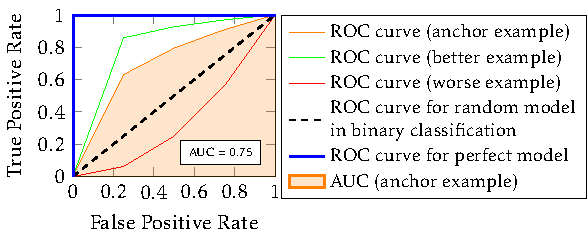
\includegraphics[page=1]{images/output-figure3.pdf}
        \caption{AUC for the anchor ROC curve}
    \end{figure}

    % \begin{figure}[H]
    %     \centering
    %     \begin{tikzpicture}
    %         \begin{axis}[ 
    %             xlabel=False Positive Rate,
    %             ylabel=True Positive Rate,
    %             xmin=0, xmax=1.0,
    %             ymin=0, ymax=1.0,
    %             xtick={0,0.2,0.4,0.6,0.8,1.0},
    %             ytick={0,0.2,0.4,0.6,0.8,1.0},
    %             legend pos=outer north east,
    %             height=0.4\textwidth,
    %             label style={font=\small},
    %             tick label style={font=\small},
    %             legend cell align={left},
    %             legend style={font=\footnotesize,
    %                         cells={align=left}}
    %           ] 
    %             \centering 
    %             \path[name path=axis] (axis cs:0,0) -- (axis cs:1,0);
    %             \addplot[domain=0:1,
    %             samples=5, color = orange, name path = anchor_roc]{x^(1/3)};
    %             \addlegendentry{ROC curve (anchor example)};
    %             \addplot[domain=0:1,
    %             samples=5, color = green, name path = better_roc]{x^(1/9)};
    %             \addlegendentry{ROC curve (better example)};
    %             \addplot[domain=0:1,
    %             samples=5, color = red, name path=worse_roc]{x^2};
    %             \addlegendentry{ROC curve (worse example)};
                
    %             \addplot[domain=0:1,
    %             samples=10, color = black, thick, dashed, name path=random_roc]{x};
    %             \addlegendentry{ROC curve for random model \\in binary classification};
    %             \addplot[domain=0:1,
    %             color = blue, {very thick}]
    %             coordinates {(0,0)(0,1)(1,1)};
    %             \addlegendentry{ROC curve for perfect model};
    %             \addplot [
    %                 thick,
    %                 color=orange,
    %                 fill=orange, 
    %                 fill opacity=0.2
    %             ]
    %             fill between[
    %                 of=anchor_roc and axis,
    %                 soft clip={domain=0:1},
    %             ];
    %             \addlegendentry{AUC (anchor example)};
    %             \node[font=\tiny,fill=white,draw,rectangle] at (axis cs: 0.73,0.15) {AUC = 0.75};
    %       \end{axis}
    %     \end{tikzpicture}
    %     \caption{AUC for the anchor ROC curve}
    % \end{figure}


\end{frame}

\begin{frame}{AUC}
    
    {\large\textbf{What is the AUC ?}}

    \begin{figure}
        \centering
        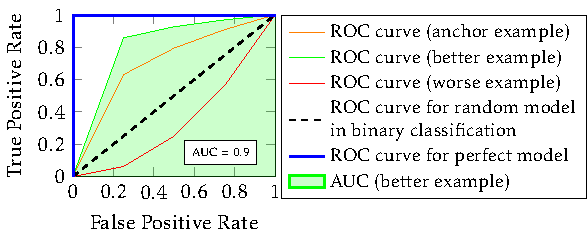
\includegraphics[page=1]{images/output-figure4.pdf}
        \caption{AUC for the better ROC curve}
    \end{figure}

    % \begin{figure}[H]
    %     \centering
    %     \begin{tikzpicture}
    %         \begin{axis}[ 
    %             xlabel=False Positive Rate,
    %             ylabel=True Positive Rate,
    %             xmin=0, xmax=1.0,
    %             ymin=0, ymax=1.0,
    %             xtick={0,0.2,0.4,0.6,0.8,1.0},
    %             ytick={0,0.2,0.4,0.6,0.8,1.0},
    %             legend pos=outer north east,
    %             height=0.4\textwidth,
    %             label style={font=\small},
    %             tick label style={font=\small},
    %             legend cell align={left},
    %             legend style={font=\footnotesize,
    %                         cells={align=left}}
    %           ] 
    %             \centering 
    %             \path[name path=axis] (axis cs:0,0) -- (axis cs:1,0);
    %             \addplot[domain=0:1,
    %             samples=5, color = orange, name path = anchor_roc]{x^(1/3)};
    %             \addlegendentry{ROC curve (anchor example)};
    %             \addplot[domain=0:1,
    %             samples=5, color = green, name path = better_roc]{x^(1/9)};
    %             \addlegendentry{ROC curve (better example)};
    %             \addplot[domain=0:1,
    %             samples=5, color = red, name path=worse_roc]{x^2};
    %             \addlegendentry{ROC curve (worse example)};
                
    %             \addplot[domain=0:1,
    %             samples=10, color = black, thick, dashed, name path=random_roc]{x};
    %             \addlegendentry{ROC curve for random model \\in binary classification};
    %             \addplot[domain=0:1,
    %             color = blue, {very thick}]
    %             coordinates {(0,0)(0,1)(1,1)};
    %             \addlegendentry{ROC curve for perfect model};
    %             \addplot [
    %                 thick,
    %                 color=green,
    %                 fill=green, 
    %                 fill opacity=0.2
    %             ]
    %             fill between[
    %                 of=better_roc and axis,
    %                 soft clip={domain=0:1},
    %             ];
    %             \addlegendentry{AUC (better example)};
    %             \node[font=\tiny,fill=white,draw,rectangle] at (axis cs: 0.73,0.15) {AUC = 0.9};
    %       \end{axis}
    %     \end{tikzpicture}
    %     \caption{AUC for the better ROC curve}
    % \end{figure}


\end{frame}


\begin{frame}{AUC}
    
    {\large\textbf{What is the AUC ?}}

    \begin{figure}
        \centering
        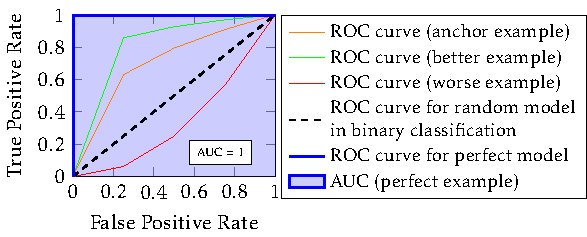
\includegraphics[page=1]{images/output-figure5.pdf}
        \caption{AUC for the perfect ROC curve}
    \end{figure}

    % \begin{figure}[H]
    %     \centering
    %     \begin{tikzpicture}
    %         \begin{axis}[ 
    %             xlabel=False Positive Rate,
    %             ylabel=True Positive Rate,
    %             xmin=0, xmax=1.0,
    %             ymin=0, ymax=1.0,
    %             xtick={0,0.2,0.4,0.6,0.8,1.0},
    %             ytick={0,0.2,0.4,0.6,0.8,1.0},
    %             legend pos=outer north east,
    %             height=0.4\textwidth,
    %             label style={font=\small},
    %             tick label style={font=\small},
    %             legend cell align={left},
    %             legend style={font=\footnotesize,
    %                         cells={align=left}}
    %           ] 
    %             \centering 
    %             \path[name path=axis] (axis cs:0,0) -- (axis cs:1,0);
    %             \addplot[domain=0:1,
    %             samples=5, color = orange, name path = anchor_roc]{x^(1/3)};
    %             \addlegendentry{ROC curve (anchor example)};
    %             \addplot[domain=0:1,
    %             samples=5, color = green, name path = better_roc]{x^(1/9)};
    %             \addlegendentry{ROC curve (better example)};
    %             \addplot[domain=0:1,
    %             samples=5, color = red, name path=worse_roc]{x^2};
    %             \addlegendentry{ROC curve (worse example)};
                
    %             \addplot[domain=0:1,
    %             samples=10, color = black, thick, dashed, name path=random_roc]{x};
    %             \addlegendentry{ROC curve for random model \\in binary classification};
    %             \addplot[domain=0:1,
    %             color = blue, {very thick}, name path = perfect_roc]
    %             coordinates {(0,0)(0,1)(1,1)};
    %             \addlegendentry{ROC curve for perfect model};
    %             \addplot [
    %                 thick,
    %                 color=blue,
    %                 fill=blue, 
    %                 fill opacity=0.2
    %             ]
    %             fill between[
    %                 of=perfect_roc and axis,
    %                 soft clip={domain=0:1},
    %             ];
    %             \addlegendentry{AUC (perfect example)};
    %             \node[font=\tiny,fill=white,draw,rectangle] at (axis cs: 0.73,0.15) {AUC = 1};
    %       \end{axis}
    %     \end{tikzpicture}
    %     \caption{AUC for the perfect ROC curve}
    % \end{figure}


\end{frame}

\subsection{ROC and bipartite ranking}
\begin{frame}{ROC and bipartite ranking}

{\large\textbf{What is the link between ROC curves and bipartite ranking ?}}

\begin{itemize}
    \item Different tasks require different metrics.
    \item \gbf{Classification} : accuracy, precision, recall, f1 score, etc.
    \item \gbf{Regression} : mean squared error, mean absolute error, etc.
    \item \textbf{None of these metrics take the rank into account.} They freeze the number of true/false positives/negatives for a \gbf{particular threshold} (usually 0.5).
    
    \end{itemize} 


\end{frame}


\begin{frame}{ROC and bipartite ranking}

\begin{itemize}
    \item  The ROC curve \gbf{intrinsically embeds the information of the rank} by giving information on the confusion matrix for all possible thresholds.
\end{itemize}

\begin{figure}
    \centering
   
    \animategraphics[autoplay,loop,width=0.7\textwidth]{2}{images/gifs/roc_curve_creation/roc_curve_creation-}{1}{21}
    % ne fonctionne que sur adobe acrobat
    
\end{figure}




\end{frame}




\begin{frame}{ROC and bipartite ranking}

    \begin{itemize}
        \item  Therefore, the analysis of the ROC curve and its AUC are \gbf{the gold standard} to assess the performance of a \gbf{bipartite ranking model}.
        \item The ROC curve and AUC can also be directly used to \gbf{learn the ranking of the instances} in bipartite ranking models.
        \item Examples for AUC optimisation : \footcite{clemencon2008ranking}\footcite{zhao2011online}
        \item Examples for ROC curve pointwise optimisation : \footcite{pmlr-v80-vogel18a} \footcite{lieberman2024optimizing}
    
    \end{itemize}
\end{frame}
        
